\documentclass[xcolor=table]{beamer}
\usetheme[progressbar=frametitle]{metropolis}
\setbeamercolor{block body}{bg=mDarkTeal!30}
\setbeamercolor{block title}{bg=mDarkTeal,fg=black!2}
\usepackage{amsmath}
\usepackage{xcolor}
\usepackage{hyperref}
\hypersetup{
colorlinks = true,
linkcolor =.,
    citecolor = .,
    urlcolor = blue
}
\usepackage{cancel}
\usepackage{amssymb}
\usepackage{comment}
\usepackage{witharrows}
\usepackage{mathtools}
\usepackage{multicol}

%21-JUN-2016


% Example definitions.
% --------------------

% Specific definitions
\def\Xtr{\mathbf{X}_{\text{tr}}}
\def\Ztr{\mathbf{Z}_{\text{tr}}}

% Packages
\usepackage{bm}
\usepackage{color}
\usepackage{amssymb}

%\usepackage{cite}
%\usepackage[pdftex]{graphicx}
\usepackage{algorithm,algorithmic}
\usepackage{amsmath}
\usepackage{url}
\usepackage{float}
\usepackage{cancel}

\usepackage{multirow}

% Functions
\def\trace{\operatorname{Tr}}
\def\KL{\mathbf{KL}}
\def\PG{\operatorname{PG}}
\newcommand{\E}{\mathbb{E}}

% Number Sets
\def\R{{\mathbb R}}
\def\Z{{\mathbb Z}}
\def\N{{\mathbb N}}

% Text
\def\p{{\mathrm{p}}}
\def\q{{\mathrm{q}}}
\def\rd{{\mathrm{d}}}

\def\F{{\mathrm{F}}}
\def\G{{\mathrm{G}}}
\def\H{{\mathrm{H}}}
\def\T{{\mathrm{T}}}

\def\KL{{\mbox{KL}}}
\def\TV{{\mbox{TV}}}

\def\tr{{\text{tr}}}

% Cal
\def\cC{{\mathcal C}}
\def\cH{{\mathcal H}}
\def\cL{{\mathcal L}}
\def\cN{{\mathcal N}}
\def\cX{{\mathcal X}}

% Bold Symbols and numbers
\def\bzero{{\mathbf 0}}
\def\bone{{\mathbf 1}}

% Greek letters
\def\balpha{{\boldsymbol{\alpha}}}
\def\bbeta{{\boldsymbol{\beta}}}
\def\bgamma{{\boldsymbol{\gamma}}}
\def\bdelta{{\boldsymbol{\delta}}}
\def\bepsilon{{\boldsymbol{\epsilon}}}
\def\bheta{{\boldsymbol{\eta}}}
\def\btheta{{\boldsymbol{\theta}}}
\def\biota{{\boldsymbol{\iota}}}
\def\bkappa{{\boldsymbol{\kappa}}}
\def\blambda{{\boldsymbol{\lambda}}}
\def\bmu{{\boldsymbol{\mu}}}
\def\bnu{{\boldsymbol{\nu}}}
\def\bxi{{\boldsymbol{\xi}}}
\def\bpi{{\boldsymbol{\pi}}}
\def\brho{{\boldsymbol{\rho}}}
\def\bsigma{{\boldsymbol{\sigma}}}
\def\btau{{\boldsymbol{\tau}}}
\def\bups{{\boldsymbol{\upsilon}}}
\def\bphi{{\boldsymbol{\phi}}}
\def\bchi{{\boldsymbol{\chi}}}
\def\bpsi{{\boldsymbol{\psi}}}
\def\bomega{{\boldsymbol{\omega}}}

\def\bAlpha{{\boldsymbol{\Alpha}}}
\def\bBeta{{\boldsymbol{\Beta}}}
\def\bGamma{{\boldsymbol{\Gamma}}}
\def\bDelta{{\boldsymbol{\Delta}}}
\def\bEpsilon{{\boldsymbol{\Epsilon}}}
\def\bHeta{{\boldsymbol{\Eta}}}
\def\bTheta{{\boldsymbol{\Theta}}}
\def\bIota{{\boldsymbol{\Iota}}}
\def\bKappa{{\boldsymbol{\Kappa}}}
\def\bLambda{{\boldsymbol{\Lambda}}}
\def\bMu{{\boldsymbol{\Mu}}}
\def\bNu{{\boldsymbol{\Nu}}}
\def\bXi{{\boldsymbol{\Xi}}}
\def\bPi{{\boldsymbol{\Pi}}}
\def\bRho{{\boldsymbol{\Rho}}}
\def\bSigma{{\boldsymbol{\Sigma}}}
\def\bTau{{\boldsymbol{\Tau}}}
\def\bUps{{\boldsymbol{\Upsilon}}}
\def\bPhi{{\boldsymbol{\Phi}}}
\def\bChi{{\boldsymbol{\Chi}}}
\def\bPsi{{\boldsymbol{\Psi}}}
\def\bOmega{{\boldsymbol{\Omega}}}

% Bold
\def\ba{{\mathbf a}}
\def\bb{{\mathbf b}}
\def\bc{{\mathbf c}}
\def\bd{{\mathbf d}}
\def\be{{\mathbf e}}
\def\bff{{\mathbf f}}
\def\bg{{\mathbf g}}
\def\bh{{\mathbf h}}
\def\bi{{\mathbf i}}
\def\bj{{\mathbf j}}
\def\bk{{\mathbf k}}
\def\bl{{\mathbf l}}
\def\bm{{\mathbf m}}
\def\bn{{\mathbf n}}
\def\bo{{\mathbf o}}
\def\bp{{\mathbf p}}
\def\bq{{\mathbf q}}
\def\br{{\mathbf r}}
\def\bs{{\mathbf s}}
\def\bt{{\mathbf t}}
\def\bu{{\mathbf u}}
\def\bv{{\mathbf v}}
\def\bw{{\mathbf w}}
\def\bx{{\mathbf x}}
\def\by{{\mathbf y}}
\def\bz{{\mathbf z}}

\def\bA{{\mathbf A}}
\def\bB{{\mathbf B}}
\def\bC{{\mathbf C}}
\def\bD{{\mathbf D}}
\def\bE{{\mathbf E}}
\def\bF{{\mathbf F}}
\def\bG{{\mathbf G}}
\def\bH{{\mathbf H}}
\def\bI{{\mathbf I}}
\def\bJ{{\mathbf J}}
\def\bK{{\mathbf K}}
\def\bL{{\mathbf L}}
\def\bM{{\mathbf M}}
\def\bN{{\mathbf N}}
\def\bO{{\mathbf O}}
\def\bP{{\mathbf P}}
\def\bQ{{\mathbf Q}}
\def\bR{{\mathbf R}}
\def\bS{{\mathbf S}}
\def\bT{{\mathbf T}}
\def\bU{{\mathbf U}}
\def\bV{{\mathbf V}}
\def\bW{{\mathbf W}}
\def\bX{{\mathbf X}}
\def\bY{{\mathbf Y}}
\def\bZ{{\mathbf Z}}

% Commands
%--------------------
\newcommand{\mean}[1]{\mathrm{<}#1\mathrm{>}}


%\newcommand{\d}{{\mathrm d}}
\DeclareMathOperator*{\diag}{diag}


% Theorems

\usepackage{amsthm}
\theoremstyle{definition}

\newtheorem{proposition}[]{Proposition}
%\newtheorem{problem}[]{Problem}

\usepackage{arydshln}
\usepackage{natbib}
 


\DeclarePairedDelimiter\abs{\lvert}{\rvert}%
\DeclarePairedDelimiter\norm{\lVert}{\rVert}%

\begin{document}

\title{Ensembles}
\subtitle{Combining continuous-valued outputs}
\author[Javier Sáez]{\textbf {Javier Sáez}} % auteur
\institute[University of Granada]{\textbf {University of Granada}\\
Visual Information Processing Group}
\date{\today}



{\setbeamertemplate{footline}{}
\begin{frame}[noframenumbering]
\titlepage
\end{frame}


\begin{frame}[noframenumbering]{Index}
\tableofcontents
\end{frame}}

%%%%%%%%%%%%%%%%%%%%
%%%%%% SECTION %%%%%
%%%%%%%%%%%%%%%%%%%%

    
\begin{frame}{Notation}
\begin{itemize}
    \item \(D_i: \R^n \to [0,1]^c\) is a classifier.
    \item \(d_{i,j}(x)\) represents the support (estimation of the posterior) that \(D_i\) gives to the hypothesis that \(\bx\) comes from class \(\omega_j\).
    \item We can build
    \[
    DP(\bx) = \begin{pmatrix}
        d_{1,1}(\bx) & \cdots & d_{1,c}(\bx)\\
        \vdots & \ddots & \vdots \\
        d_{L,1}(\bx) & \cdots & d_{L,c}(\bx)
    \end{pmatrix}.
    \]
    \item And calculate a degree of support for class \(\omega_j\):
    \[
    \mathbf{\mu}_j(\bx) = \mathbf{\mathcal F}\left(d_{1,j}(\bx),\cdots, d_{L,j}(\bx)\right).
    \]
    We label \(\bx\) as the class with the largest support.
\end{itemize}

\vspace{1cm}
Book: 
    \cite{10.5555/2935490}
\end{frame}



%%%%%%%%%%%%%%%%%%%%
%%%%%% SECTION %%%%%
%%%%%%%%%%%%%%%%%%%%

\section{Generic Formulation}
\begin{frame}{Simple non-trainable combiners}
The most common combiners are:
\begin{itemize}
    \item  Average (sum)
    \[
    \mu_j(\bx) = \frac{1}{L}\sum_{i=1}^L d_{i,j}(\bx)
    \]
    \item Max/min/median of the 
    \[
    \mu_j(\bx) = \max_i \{d_{i,j}(\bx)\}.
    \]
    \item Trimmed mean: sort \(d_{i,j}\) and remove \(K/2\%\) from each side, and then compute \(\mu_j(\bx)\) as the average of the rest.
    \item Product combiner/ geometric mean:
    \[
    \mu_j(\bx) = \left(\prod_{i=1}^L d_{i,j}(\bx)\right)^{1/L}
    \]
\end{itemize}
    All these are non trainable.
\end{frame}

\subsection{Equivalences}


\begin{frame}{Equivalences}
\begin{proposition}
    Let \(a_1,\dots,a_L\) be the outputs for class \(\omega_1\) and \(1-a_1,\dots,1-a_L\) the outputs for class \(\omega_2\), \(a_i\in[0,1]\). Then, the class label assigned to \(\bx\) by the MAX and MIN combination rules is the same.
    \end{proposition}
    \pause
        \begin{proposition}
    Let \(L\) be an odd natural number. Let \(a_1,\dots,a_L\) be the outputs for class \(\omega_1\) and \(1-a_1,\dots,1-a_L\) the outputs for class \(\omega_2\), \(a_i\in[0,1]\). Then, the class label assigned to \(\bx\) by the Majority Vote and Median combination rules is the same.
    \end{proposition}
\end{frame}

%%%%%%%%%%%%%%%%%%%%
%%%%%% SECTION %%%%%
%%%%%%%%%%%%%%%%%%%%

\section{Generalized Mean Combiner}
\begin{frame}{Generalized Mean Combiner}
\begin{definition}
    The \textbf{generalized mean combiner} assigns to each class \(\omega_j\) the support:
    \[
    \mu_j(\bx,\alpha) = \left( \frac{1}{L} \sum_{i=1}^L d_{i,j}(\bx)^\alpha \right)^{\frac{1}{\alpha}}
    \]
\end{definition}

\pause

Of course, \(\alpha\) can be trained! 


\end{frame}




\begin{frame}{Special cases}
\begin{itemize}
\item \(\alpha \to \infty \implies \mu_j(\bx,\alpha)\) is the maximum combiner.\\
    \pause
    \only<2>{Let \(d_*\) be the maximum of \(d_{i,j}\) for \(i = 1,\dots,L\).
    \begin{align*}\lim_{\alpha \to \infty} \log \mu_j(\bx,\alpha) & = \lim_{\alpha \to \infty} \frac{1}{\alpha} \log \frac{\sum_{i=1}^L d_{i,j}^\alpha}{L} \\
    & = \log d_* +\lim_{\alpha \to \infty} \frac{1}{\alpha} \log \frac{\sum_{i=1}^L \left(\frac{d_{i,j}}{d_*}\right)^\alpha}{L}\\
    & = \log d_*
    \end{align*}}
    \pause
    
    \item \(\alpha = 1 \implies \mu_j(\bx,\alpha) = \frac{1}{L} \sum_{i=1}^L d_{i,j}\) is the arithmetic mean.
    \item \(\alpha \to 0 \implies \mu_j(\bx,\alpha) = \left(\prod_{i=1}^L d_{i,j}\right)^{\frac{1}{L}}\) is the geometric mean.
    \item \(\alpha = -1 \implies \mu_j(\bx,\alpha) = \left( \frac{1}{L} \sum_{i=1}^L \frac{1}{d_{i,j}(\bx)} \right)^{-1} \) is the harmonic mean.
    
    
    \item \(\alpha \to -\infty \implies \mu_j(\bx,\alpha)\) is the minimum combiner.\\
\end{itemize}

\pause

\(\alpha\) can then be understood as the level of \emph{optimism} of the \textbf{combiner}:
\begin{itemize}
    \item \(\alpha \to -\infty\) is the most pessimistic, implying that \textbf{all} the classifiers must agree with the choice (minimum combiner).
    \item \(\alpha \to \infty\) is the most optimistic (maximum combiner), where \textbf{at least one} of the classifiers supports \(\omega_j\).
\end{itemize} 
    
\end{frame}
%%%%%%%%%%%%%%%%%%%%
%%%%%% SECTION %%%%%
%%%%%%%%%%%%%%%%%%%%

\section{Theoretical Comparison of Simple combiners}

\begin{frame}{Scenario}

Let us consider the following scenario:

\begin{itemize}
    \item There are only two classes \(\Omega = \{\omega_1, \omega_2\}\).
    \item We assume that \(d_{j,i}(\bx)\) is an estimate of the posterior \(p(\omega_i\mid \bx)\) produced by the classifier \(D_j\) and that, for any \(\bx\),
    \[
    d_{j,1}(\bx) + d_{j,2}(\bx) = 1.
    \]
    \item We assume without loss of generality that the true posterior probability is
    \[
    p(\omega_1 \mid \bx) = p > 0.5,
    \]
    so Bayes-optimal class label for \(\bx\) is \(\omega_1\) (and assigning \(\omega_2\) is a classification error).
\end{itemize}
\end{frame}


\begin{frame}{Assumption}
    The classifiers commit i.i.d. errors in estimating \(p(\omega_1 \mid \bx)\) such that:
    \[
    P_j \equiv d_{j,1}(\bx) = p(\omega_1\mid \bx) + \eta(\bx) = p + \eta(\bx)
    \]
    and
    \[
    d_{j,2}(\bx) = 1 - p - \eta(\bx),
    \]
    where \(\eta(\bx)\) is often:
    \begin{itemize}
        \item a Gaussian distribution \(\eta(\bx) \sim \mathcal N (0,\sigma^2)\) or
        \item a continuous uniform distribution \(\eta(\bx) \sim U([-b,b])\).
    \end{itemize}

\pause
    Thus, \(d_{j,i}(\bx)\) are random variables. Using the fusion method \(\mathcal F\), the posterior estimates are:
    \[
    \hat P_1 = \mathcal F \left(P_1,\dots, P_L\right), \quad \hat P_2 = \mathcal F \left(1-P_1,\dots, 1-P_L\right)
    \]
\end{frame}


\begin{frame}{Errors}
    \begin{itemize}
        \item For the single classifier, average and median fusion models \(\hat P_1 + \hat P_2 = 1\). Thus, if \(\omega_1\) is the correct label, it is sufficient to have \(\hat P_1 > 0.5\) to label \(\bx\) as \(\omega_1\).\\
        The probability of error is then:
        \[
        P_e = P(\hat P_1 \leq 0.5) = F_{\hat P_1}(0.5) = \int_0^{0.5}f_{\hat P_1}(y) dy
        \]
        \pause
        \item For the minimum and maximum rules, \(\hat P_1 + \hat P_2 \neq 1\) necessarily. An error occurs if \(\hat P_1 \leq \hat P_2\):
        \[
        P_e = P(\hat P_1 \leq \hat P_2).
        \]
    \end{itemize}
\end{frame}


\begin{frame}{Individual Error}

Using a Gaussian distribution, \(\hat P_1 \sim \mathcal N(p,\sigma^2)\). Denoting by \(\Phi(z)\) to the C.D.F. of the \(\mathcal N(0,1)\), then
\[
F(t) = \Phi\left( \frac{t-p}{\sigma}\right).
\]
\pause
Since \(F_{\hat P_1}(t) = F(t)\), \textbf{individual error} of a classifier is:
\[
P_e = \Phi\left( \frac{0.5-p}{\sigma}\right).
\]
    
\end{frame}

\begin{frame}{Average combiner error}

Given that \(\hat P_1 = \frac{1}{L}  \sum_{j=1}^L P_j\), since \(P_j\) are normally distributed and independent, then \(\hat P_1 \sim \mathcal N \left(p, \frac{\sigma^2}{L}\right)\). Hence, the probability of error in this case is:
\[
P_e = P(\hat P_1 < 0.5) = \Phi \left( \frac{\sqrt{L} (0.5 - p)}{\sigma}\right)
\]
    
\end{frame}

\begin{frame}{Median / Majority vote error}
    In the median fusion method:
    \[
    \hat P_1 = \text{med} \{ P_1,\dots,P_L\} = p + \text{med}\{\eta_1,\dots,\eta_L\} = p + \eta_m. 
    \]
    \pause
    The probability of error is:
    \[
    P_e = P(p + \eta_m < 0.5) = P(\eta_m < 0.5 - p) = F_{\eta_m}(0.5 - p)
    \]
    \pause
    From order statistics theory \citep{mood1973introduction}
    \[
    F_{\eta_m}(t) = \sum_{j = \frac{L+1}{2}}^L \binom{L}{j} F_\eta(t)^j[1-F_\eta(t)]^{L-j}
    \]
\end{frame}


\begin{frame}{Median / Majority vote error}
    Using that \(\eta\) follows a Gaussian distribution, the probability of error is:
    \[
    P_e =  \sum_{j = \frac{L+1}{2}}^L \binom{L}{j} \Phi\left(\frac{0.5-p}{\sigma}\right)^j \left[1-\Phi\left(\frac{0.5-p}{\sigma}\right)^j\right]^{L-j}
    \]
\end{frame}

\begin{frame}{Visual Comparison}
    \begin{figure}
        \centering
        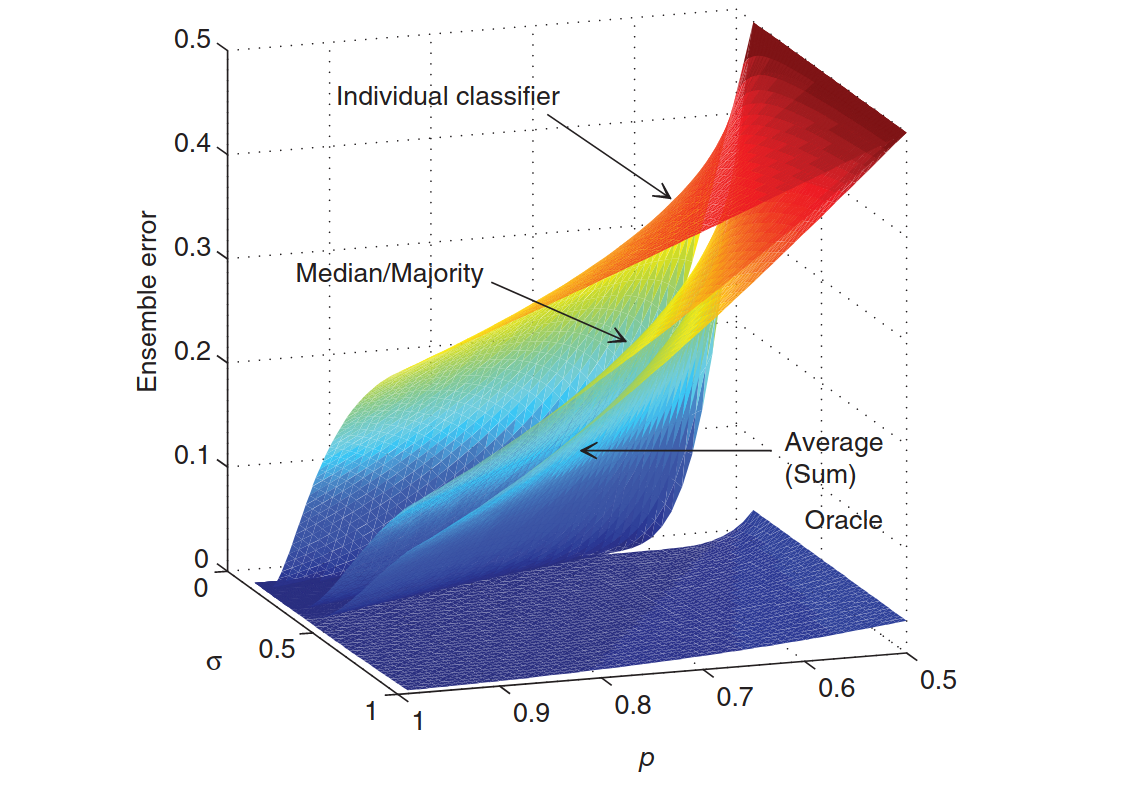
\includegraphics[scale=0.22]{Presentations/Images/error_surface.png}
        \caption{Theoretical of the Majority Vote and Average ensembles.}
    \end{figure}
\end{frame}
%%%%%%%%%%%%%%%%%%%%
%%%%%% SECTION %%%%%
%%%%%%%%%%%%%%%%%%%%

\section{Theoretical framework for the product combiner}

\begin{frame}{Scenario}
    \begin{itemize}

        \item Since \(d_{i,j}\) is an estimate of  \(p(\omega_j \mid \bx, D_i)\), each classifier \(D_i\) produces a probability distribution on the set of classes \(\Omega\). We name this distribution \(P_{(i)} = (d_{i,1}(\bx),\dots,d_{i,c}(\bx))\).
        \pause
        \item Also, the combiner produces a probability distribution \(P_{ens} = (\mu_1(\bx), \dots,\mu_c(\bx))\).
        \pause
        \item We would like our combiner to agree with the decisions of the classifiers, that is, we would like the probability distributions to be similar.
        \pause
        \item The KL-divergence measures the similarity between probability distributions
    \end{itemize}
    \pause
    The average KL divergence across the \(L\) members is:
    \[
    \text{KL}_{av} = \frac{1}{L} \sum_{i=1}^L \text{KL}(P_{ens} \parallel P_{(i)})
    \]
\end{frame}

\begin{frame}{Minimization}
    \begin{problem}
    \[
    \min_{P_{ens}} KL_{av}\quad s.t. \quad \sum_{k=1}^c \mu_k = 1
    \]
    \end{problem}
    \pause
    We solve it using its Lagrangian:
    \\
    \[
    \mathcal L (\{\mu_i\}_{i=1}^c, \lambda) = KL_{av} + \lambda \left(1 + \sum_{k=1}^c \mu_k\right)
    \]
    
\end{frame}

\begin{frame}{Minimization}
Recalling that 
\[
KL(p \parallel q) = \sum_{x}p(x) \log_2 \left(\frac{p(x)}{q(x)}\right),
\]
\pause
We derivate \(\mathcal L\) w.r.t. each of its parameters to find its minimum:
\begin{align*}
\frac{\partial \mathcal L}{\partial \mu_j} & = \frac{\partial}{\partial \mu_j} \left[ KL_{av} + \lambda \left(1 - \sum_{k=1}^c \mu_k\right)\right]\\
& = \frac{1}{L} \sum_{i=1}^L \frac{\partial}{\partial \mu_j} \left[\sum_{k=1}^c\mu_k \log_2 \left(\frac{\mu_k}{d_{i,k}}\right)\right] - \lambda\\
& = \frac{1}{L} \sum_{i=1}^L \left(\log_2 \left(\frac{\mu_j}{d_{i,j}}\right) + C\right) - \lambda = 0,
\end{align*}
with \(C = \frac{1}{ln(2)}\).
\end{frame}

\begin{frame}{Minimization}
    Solving for \(\mu_j\), we obtain:
    \[
    \mu_j = 2^{(\lambda - C)} \prod_{i=1}^L (d_{i,j})^{1/L}.
    \]
    Using in that expression our problem constraint, we obtain:
    \[
    \lambda = C - \log_2 \left(\sum_{k=1}^c \prod_{i=1}^L (d_{i,k})^{1/L}\right),
    \]
    \pause
    which leads to the final expression:
    \[
    \mu_j = \frac{\prod_{i=1}^L(d_{i,j})^{1/L}}{\sum_{k=1}^c \prod_{i=1}^L (d_{i,k})^{1/L}}.
    \]
    which is the normalized \textbf{geometric mean}.
\end{frame}

\begin{frame}{Average combiner}

\begin{itemize}
    \item KL-divergence is not symmetric!
    \item If instead we wrote
    \[
    KL (P_{(i)} \parallel P_{ens}),
    \]
    and we repeat the process we obtain that \(\mu_j\) is the average combiner.
\end{itemize}
    
\end{frame}
%%%%%%%%%%%%%%%%%%%%
%%%%%% SECTION %%%%%
%%%%%%%%%%%%%%%%%%%%

\begin{frame}{}
    \begin{center}
        Thank you for your attention
    \end{center}
\end{frame}




  \begin{frame}[noframenumbering]{Bibliography}

  %\vspace{0.5cm}
  \bibliographystyle{unsrtnat}
  \bibliography{bibliography.bib}

  \end{frame}

  \section*{Appendix}

  \begin{frame}{Equivalence between Min and Max for 2 classes}
    \begin{proposition}
    Let \(a_1,\dots,a_L\) be the outputs for class \(\omega_1\) and \(1-a_1,\dots,1-a_L\) the outputs for class \(\omega_2\), \(a_i\in[0,1]\). Then, the class label assigned to \(\bx\) by the MAX and MIN combination rules is the same.
    \end{proposition}
    \pause
    Assume \(a_1 = \min_i a_i\) and \(a_L = \max_i a_i\). 
    \begin{itemize}
        \item Minimum will choose \(\mu_1(\bx) = a_1\) and \(\mu_2(\bx) = 1-a_L\)
        \item Maximum will choose \(\mu_1(\bx) = a_L\) and \(\mu_2(\bx) = 1-a_1\)
    \end{itemize}
    \pause
Then,
    \begin{itemize}
        \item \(a_1 > 1- a_L\ \implies a_L < 1- a_1\) both methods choose \(\omega_1\)
        \item \(a_1 < 1- a_L \implies a_L < 1- a_1\) both methods choose \(\omega _2\)
        \item \(a_1 = 1- a_L\) both methods choose randomly
    \end{itemize}
\end{frame}


\begin{frame}{Equivalence Between Majority Vote and Median for 2 classes}
    \begin{proposition}
    Let \(L\) be an odd natural number. Let \(a_1,\dots,a_L\) be the outputs for class \(\omega_1\) and \(1-a_1,\dots,1-a_L\) the outputs for class \(\omega_2\), \(a_i\in[0,1]\). Then, the class label assigned to \(\bx\) by the Majority Vote and Median combination rules is the same.
    \end{proposition}
    \pause
    Assume \(a_1 = \min_i a_i\) and \(a_L = \max_i a_i\). The median of the outputs for class \(\omega_1\) is \(a_{\frac{L+1}{2}} = m\).
    \begin{itemize}
        \item If \(m > 0.5\), the median of the outputs for \(\omega_2\) is \(1- m < 0.5\), so \(\omega_1\) is selected. This means that at least \(\frac{L+1}{2}\) posterior probabilities for \(\omega_1\) were greater than \(0.5\), so the majority vote also assigns \(\omega_1\) to \(\bx\)
        \item If \(m < 0.5\), then \(1- m > 0.5\) and the median assigns \(\omega_2\), but also \(\frac{L+1}{2}\) posteriors for \(\omega_2\) are greater than \(0.5\), so Majority vote also assigns \(\omega_2\) to \(\bx\)
    \end{itemize}
\end{frame}


\begin{frame}{Proof \(F_{\eta_m}\)}
    \begin{theorem}[Theorem 11, page 252 \cite{mood1973introduction}]
    Let \(Y_1\leq Y_2 \leq \dots \leq Y_n\) represent the order statistics from a c.d.f. \(F\). The marginal c.d.f. of \(Y_\alpha\) is:
    \[
    F_{Y_\alpha}(y) =  \sum_{j = \alpha}^n \binom{n}{j} F_\eta(t)^j[1-F_\eta(t)]^{n-j}
    \]
    \end{theorem}
    Proof: For a fixed \(y\), let \(Z_i = I_{(-\infty,y)}(X_i)\). Then \(\sum_{i=1}^n Z_i\) is the number of \(X_i\) that are lesser or equal than \(y\). Note that \(\sum_i Z_i\) follows a binomial distribution with parameters \(n\) and \(F(y)\). Thus,
    \[
    F_{Y_\alpha}(y) = P[Y_\alpha \leq y] = P\left[\sum_i Z_i \geq \alpha\right] = \sum_{j = \alpha}^n \binom{n}{j} F_\eta(t)^j[1-F_\eta(t)]^{n-j}
    \]
\end{frame}
\end{document}